\documentclass[aspectratio=169,10pt]{beamer}

% ==========================================================
% Super deck for Munich (45 min clean talk) + TU/e subset
% ----------------------------------------------------------
% Compile (from repo root):
%   pdflatex superdeck.tex
%
% To generate the TU/e short version:
%   set \shorttrue below.
% ==========================================================

% ---- Toggle short version (TU/e) ----
\newif\ifshort
\shortfalse      % Munich (45 min clean talk)
% \shorttrue     % TU/e (20 min clean talk)

% ---- Theme / look ----
\usetheme{Madrid}
\usecolortheme{beaver}
\setbeamertemplate{navigation symbols}{}
\setbeamertemplate{footline}[frame number]
\setbeamerfont{title}{series=\bfseries}
\setbeamerfont{frametitle}{series=\bfseries}

% ---- Packages ----
\usepackage[T1]{fontenc}
\usepackage[utf8]{inputenc}
\usepackage{graphicx}
\usepackage{booktabs}
\usepackage{amsmath,amssymb}
\usepackage{mathtools}
\usepackage{xcolor}
\usepackage{pifont}
\usepackage{tikz}
\usetikzlibrary{arrows.meta,positioning,shapes.geometric,calc}
\usepackage{hyperref}

% ---- Paths to existing figures in this repo ----
\graphicspath{
  {Business_Process_Optimization/figs/}
  {ICAPS_problem_definition_final/images/}
  {IJCAI2026_Learn_to_Schedule/}
  {IJCAI2026_Learn_to_Schedule/images_appendix/}
}

% ---- Small helpers ----
\newcommand{\cmark}{\ding{51}}
\newcommand{\xmark}{\ding{55}}
\newcommand{\btext}[1]{\textbf{\color{darkred}#1}}
\definecolor{darkred}{RGB}{140,0,0}
\definecolor{darkgray}{RGB}{60,60,60}

% ---- Section slides ----
\AtBeginSection[]{
  \begin{frame}{Roadmap}
    \tableofcontents[currentsection,hideothersubsections]
  \end{frame}
}

% ==========================================================
% Title
% ==========================================================
\title[AI for BPO Scheduling]{AI for Business Process Optimization:\\From Proactive Scheduling to Decision-Focused Learning}
\author[Arik Senderovich]{Arik Senderovich}
\institute[York University]{York University}
\date{January 2026}

\begin{document}

\begin{frame}
  \titlepage
  \vspace{-0.3cm}
  \begin{center}
    \small
    \color{darkgray}
    \ifshort
Eindhoven University of Technology
    \else
Technical University of Munich
    \fi
  \end{center}
\end{frame}

% ==========================================================
% 1) Motivation + framing (BPO)
% ==========================================================
\section{Motivation: BPO as decision-making under uncertainty}

\begin{frame}{BPO in one picture: a process with decision points}
  \begin{center}
    % Make the BPMN visual dominant (readable in a large room).
    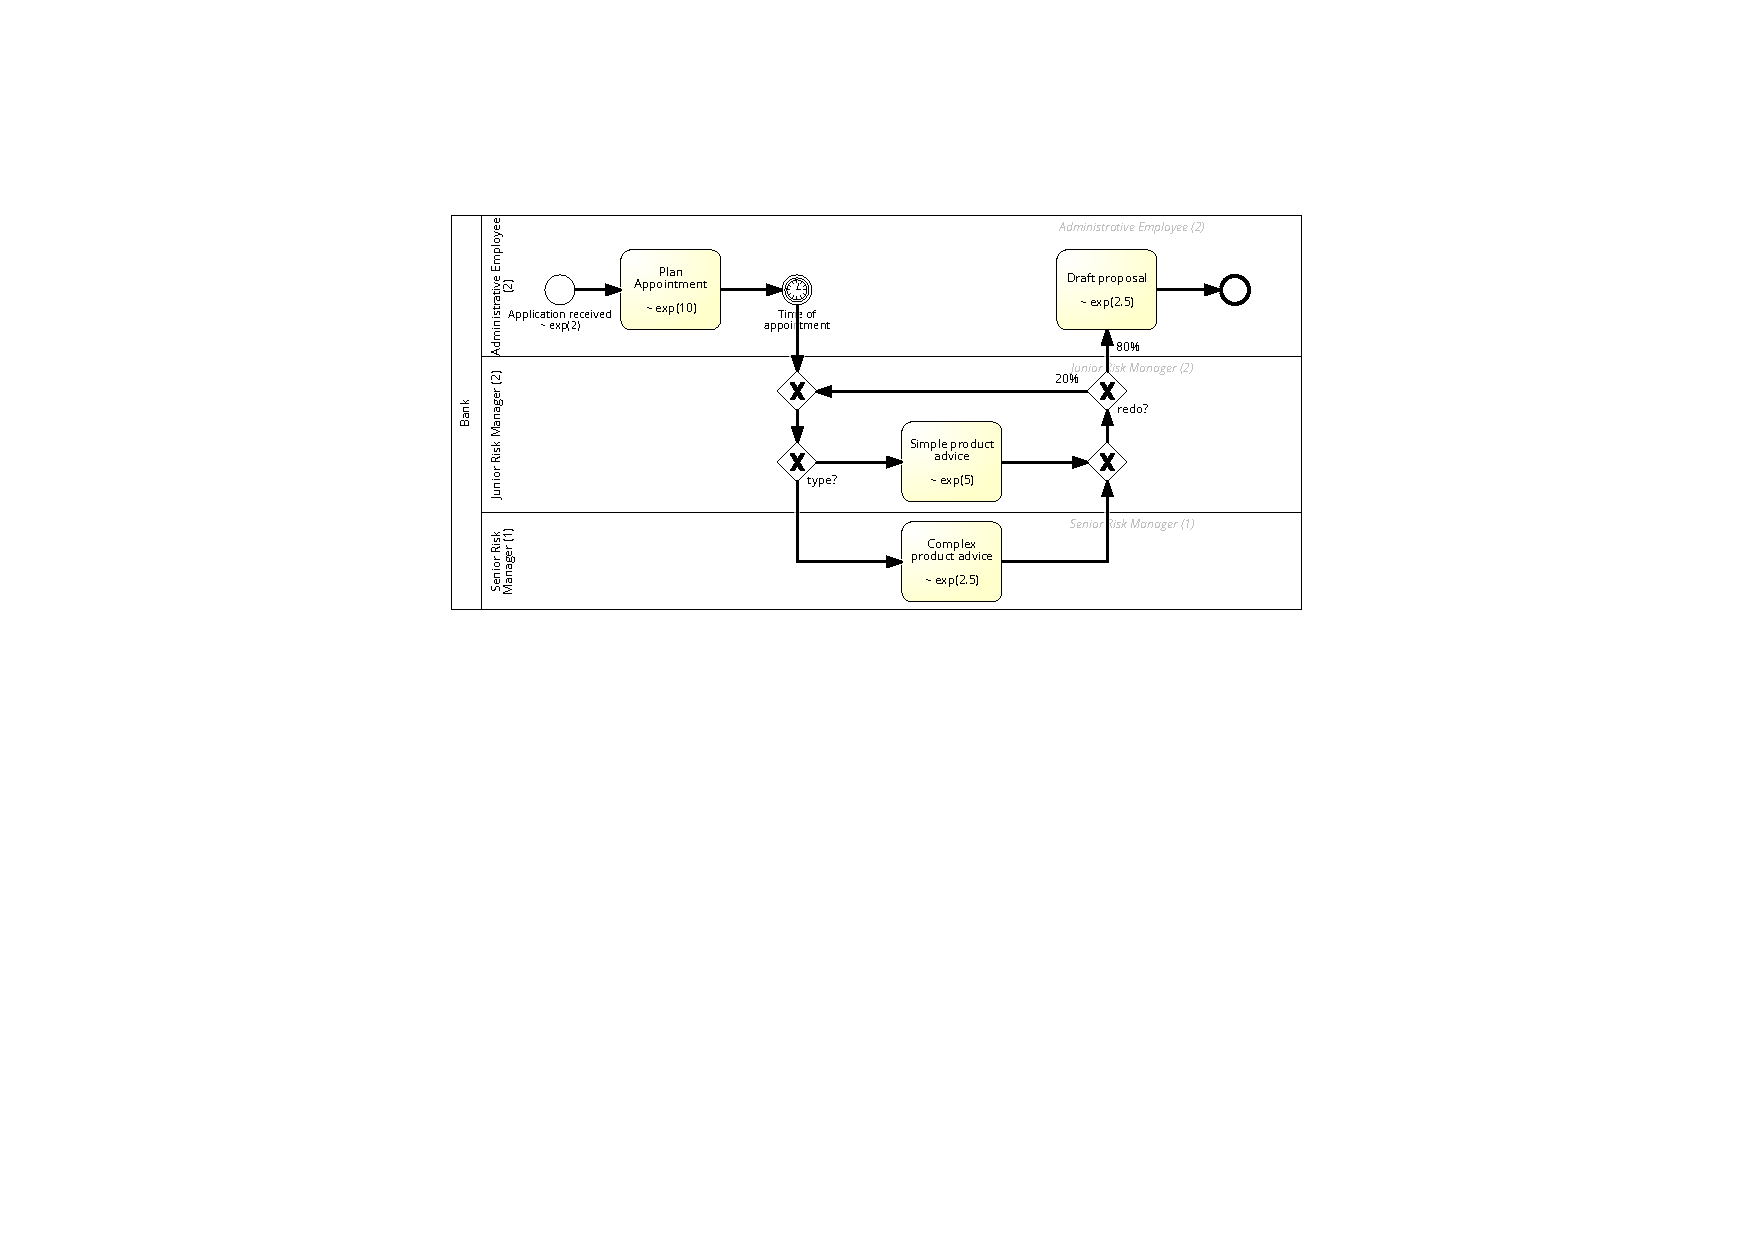
\includegraphics[width=0.98\textwidth,height=0.78\textheight,keepaspectratio]{process.pdf}
  \end{center}
  \vspace{-0.15cm}
  \scriptsize
  \color{darkgray}
  Example: a single process model already contains multiple BPO decision points (appointment, routing, rework trade-offs).
\end{frame}

\begin{frame}{What is Business Process Optimization (BPO)?}
  \begin{columns}[T]
    \column{0.72\textwidth}
      \btext{BPO} = making \emph{optimal} operational decisions during process execution
      (and designing policies for them).

      \vspace{0.35cm}
      \begin{itemize}
        \item \btext{Decisions}: \emph{what to do next} and \emph{with which resources}.
        \item \btext{Objectives}: time, cost, throughput, service levels, customer experience.
        \item \btext{Constraints}: capacity, calendars, deadlines, policies.
        \item \btext{Hard part}: uncertainty in arrivals, durations, and paths.
      \end{itemize}

      \vspace{0.15cm}
      \small
      In a moment, we’ll zoom in on \btext{scheduling} as a canonical BPO problem.

    \column{0.28\textwidth}
      \centering
      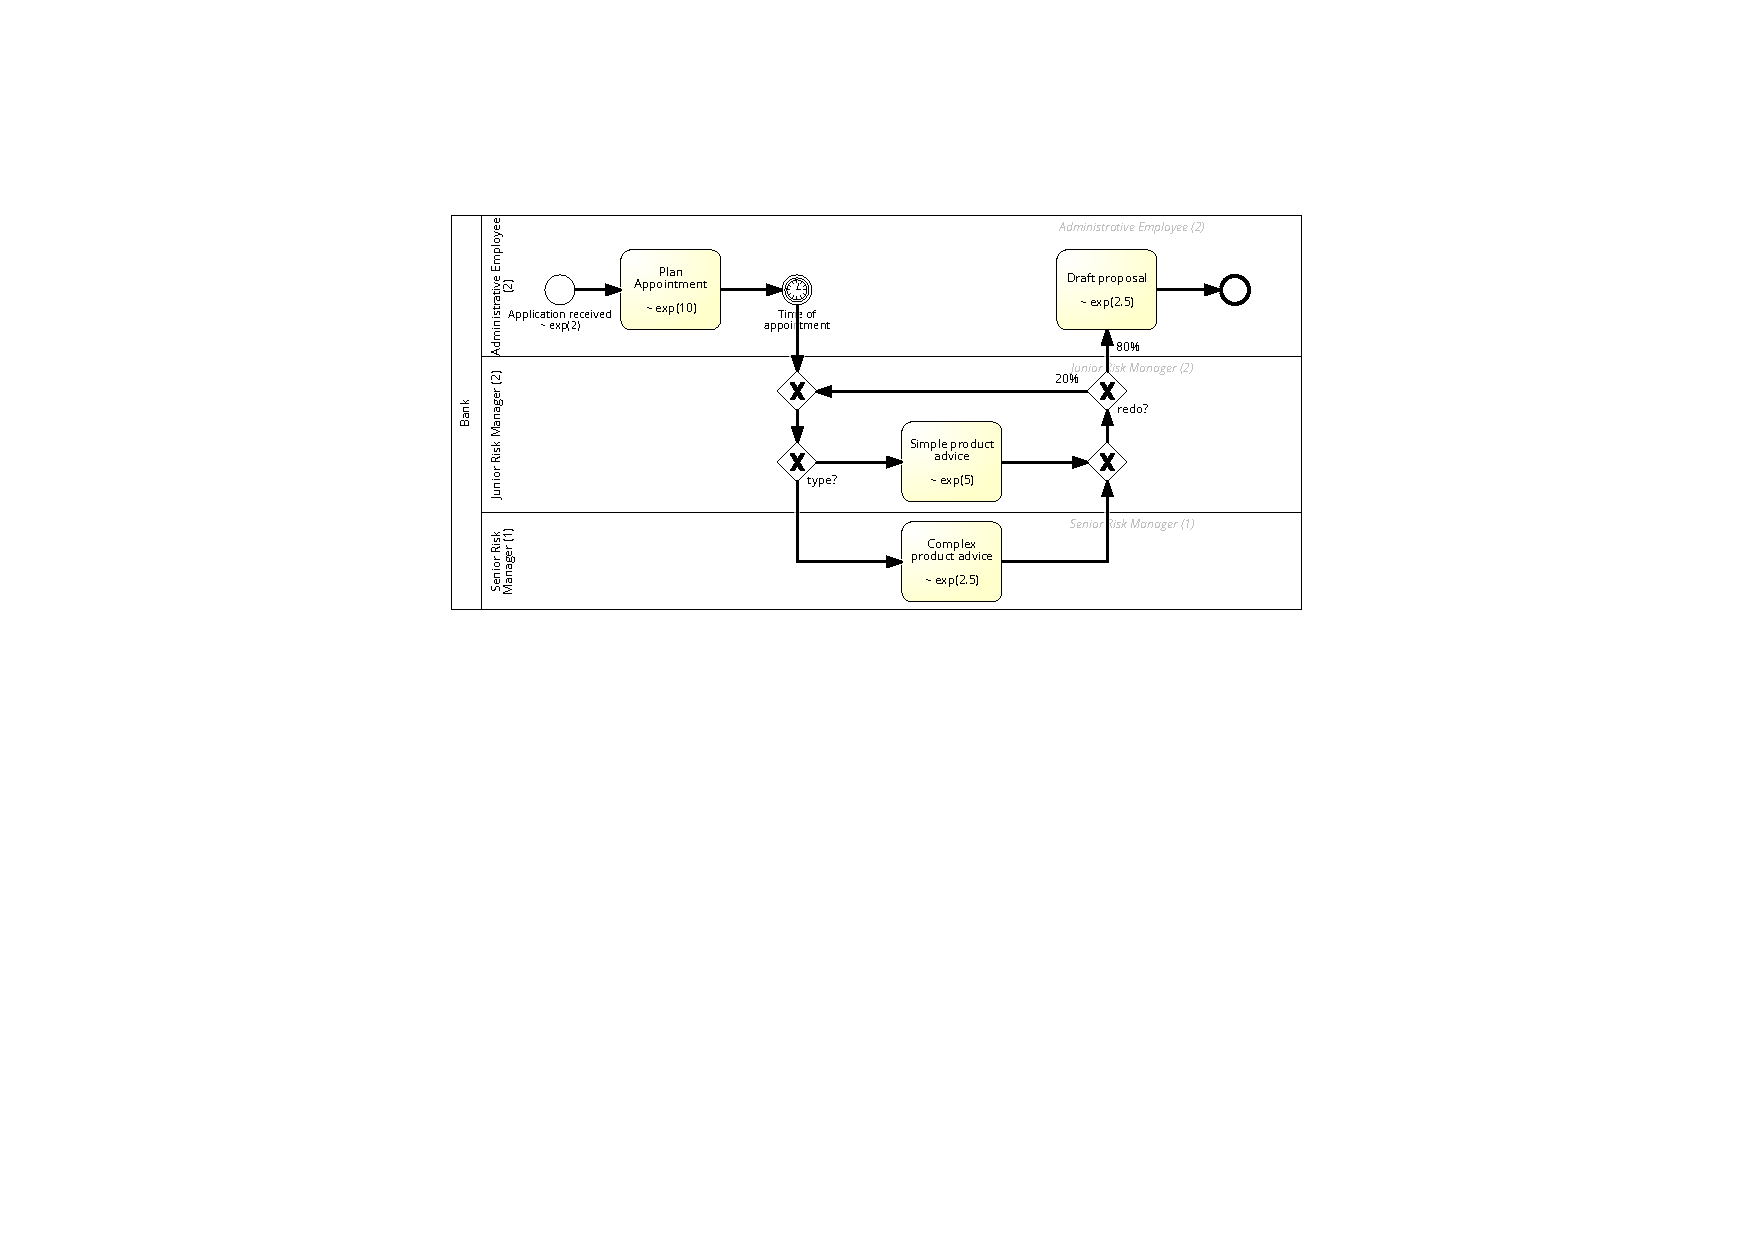
\includegraphics[width=\textwidth]{process.pdf}
      \vspace{0.1cm}
      \scriptsize
      A running process example.
  \end{columns}
\end{frame}

\begin{frame}{How do we solve BPO problems? (a reusable blueprint)}
  \begin{center}
    % Constrain height to avoid cropping on 16:9 projectors.
    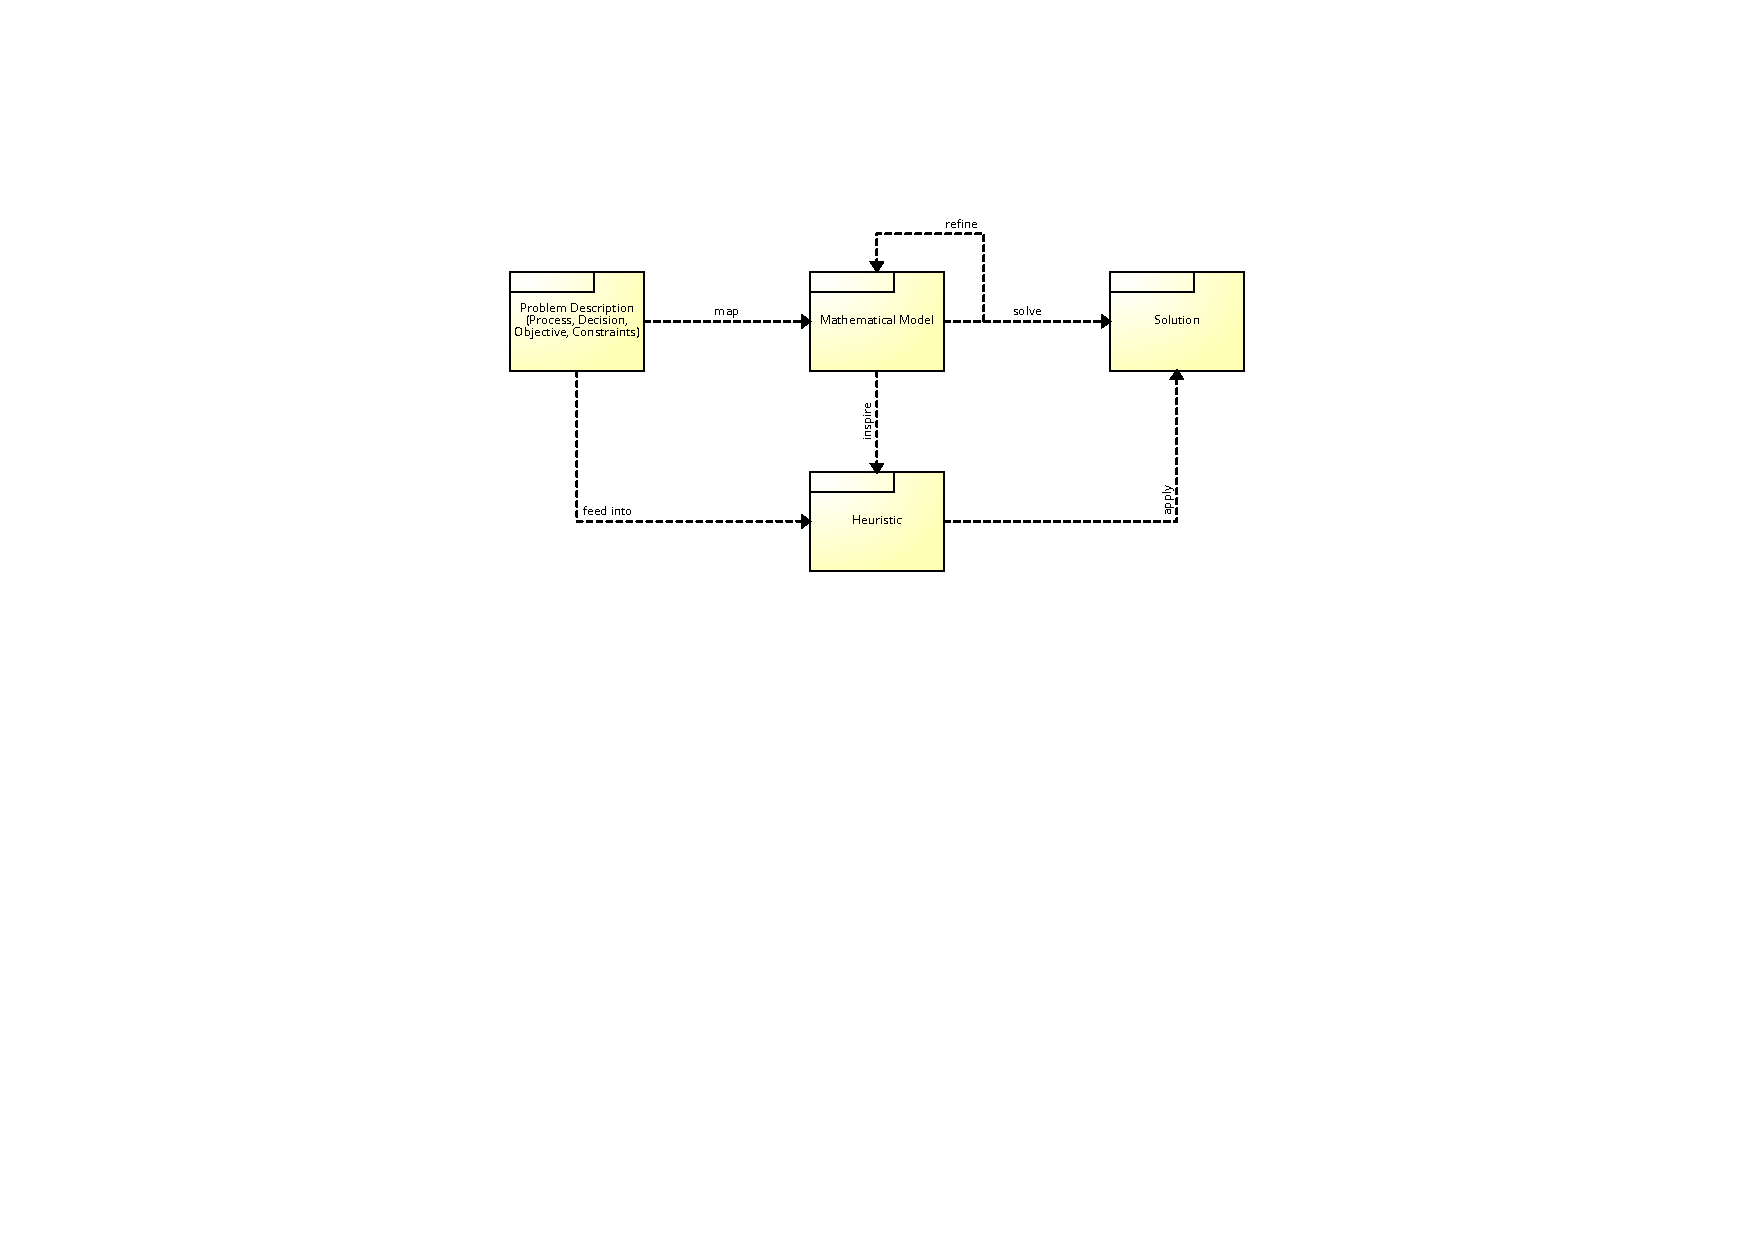
\includegraphics[width=0.90\textwidth,height=0.56\textheight,keepaspectratio]{framework.pdf}
  \end{center}
  \vspace{-0.1cm}
  \begin{columns}[T]
    \column{0.5\textwidth}
      \begin{itemize}
        \item \btext{Problem description}: decision, objective, constraints, state
        \item \btext{Data \& uncertainty}: event logs $\rightarrow$ distributions/calendars
      \end{itemize}
    \column{0.5\textwidth}
      \begin{itemize}
        \item \btext{Modeling}: CP/MIP/queues/MDPs (as appropriate)
        \item \btext{Method \& evaluation}: solve/heuristics + simulation/replay
      \end{itemize}
  \end{columns}
\end{frame}

\begin{frame}{Why scheduling in business processes is different}
  \begin{itemize}
    \item \btext{Uncertainty}: human-driven durations + stochastic variability.
    \item \btext{Planned unavailability}: calendars, shifts, vacations, partial capacity.
    \item \btext{Process structure}: precedence constraints from control-flow; multiple cases; routing.
    \item \btext{Data gap}: parameters are rarely ``given''; we infer them from event logs.
  \end{itemize}

  \vspace{0.4cm}
  \begin{block}{Talk roadmap (two lenses)}
    \begin{enumerate}
      \item \btext{Proactive scheduling from logs} (robust plans under uncertainty + calendars).
      \item \btext{Predict-and-schedule} (learn predictions that \emph{directly} improve schedules).
      \ifshort\else
      \item \btext{Teaser}: why OR-gateways create synchronization externalities.
      \fi
    \end{enumerate}
  \end{block}
\end{frame}

% ==========================================================
% 2) IJCAI'25 Proactive BPSP
% ==========================================================
\section{Lens 1: Proactive scheduling of business processes from event logs}

\begin{frame}{A simple taxonomy of BPO problem types (operational level)}
  \begin{columns}[T]
    \column{0.68\textwidth}
      \begin{itemize}
        \item \btext{Task prioritization} \& \btext{resource allocation} (dispatching)
        \item \btext{Case admission} \& \btext{case scheduling} \hfill \btext{(focus today)}
        \item \btext{Staffing} (dynamic capacity decisions)
        \item \btext{Path choice} (routing / treatment options)
      \end{itemize}

      \vspace{0.35cm}
      \begin{block}{Today’s focus}
        Scheduling: turning a BPM model + data into concrete, robust operational plans.
      \end{block}

    \column{0.32\textwidth}
      \centering
      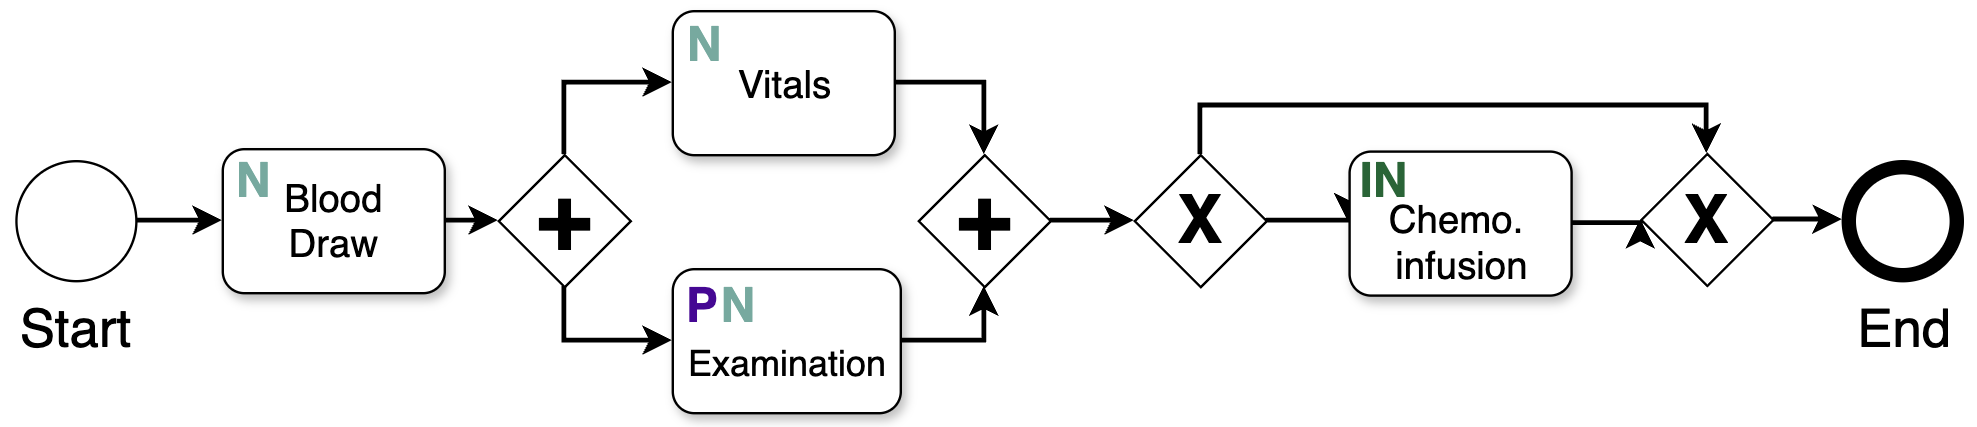
\includegraphics[width=\textwidth]{bpmn.png}
      \vspace{0.1cm}
      \scriptsize
      A process induces precedence and resource constraints.
  \end{columns}
\end{frame}

\begin{frame}{Problem: Proactive Business Process Scheduling (BPSP)}
  \begin{columns}[T]
    \column{0.6\textwidth}
      \btext{Input}:
      \begin{itemize}
        \item process structure + precedence constraints
        \item resources with \btext{calendars} / capacities
        \item stochastic activity durations (from event logs)
      \end{itemize}
      \vspace{0.2cm}
      \btext{Decision}: build a schedule that is \btext{robust} to duration uncertainty.

      \vspace{0.2cm}
      \btext{Goal}: minimize probabilistic makespan \(M_\alpha^\star\)
      (e.g., 95th percentile completion time).

    \column{0.4\textwidth}
      \centering
      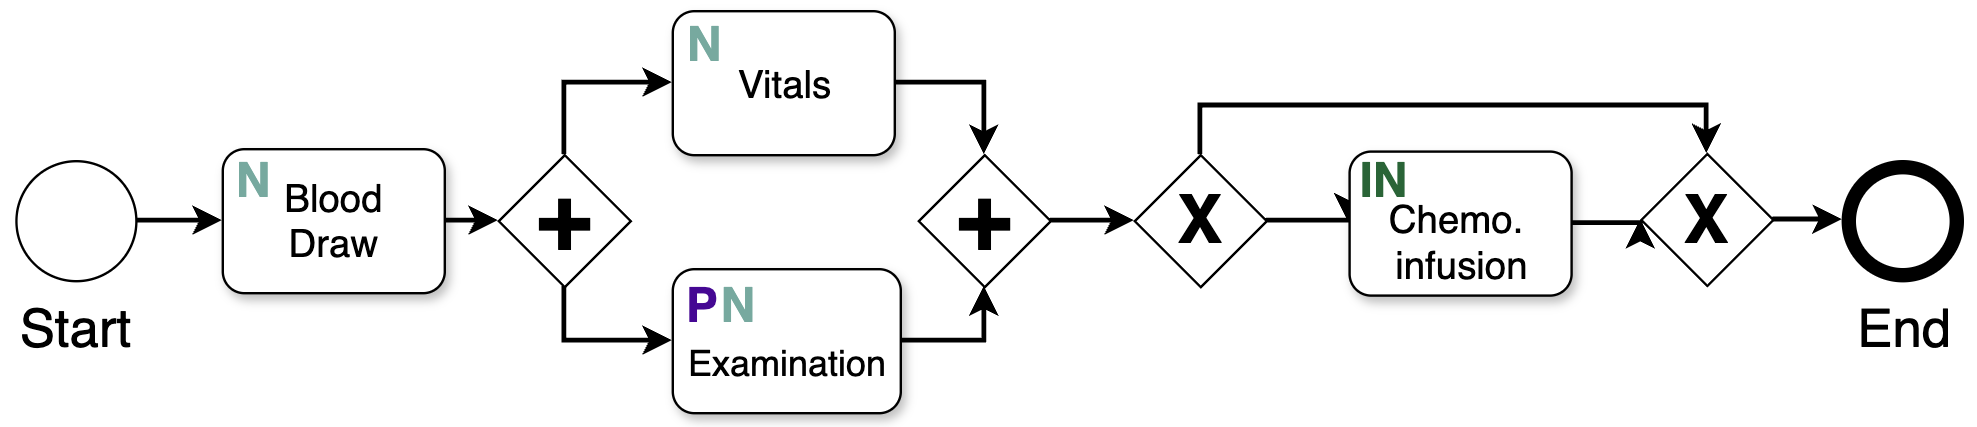
\includegraphics[width=\textwidth]{bpmn.png}
      \scriptsize
      A process induces precedence and resource constraints.
      % Placeholder idea: add a small "calendar" icon overlay in the final deck.
  \end{columns}
\end{frame}

\begin{frame}{BPSP research landscape: where does this sit?}
  \begin{columns}[T]
    \column{0.62\textwidth}
      \begin{block}{Three communities, three partial answers}
        \begin{itemize}
          \item \btext{BPM/BPO}: control-flow + event logs, but limited scheduling realism
          \item \btext{Scheduling/OR}: strong models/algorithms, often assumes parameters are given
          \item \btext{Proactive/robust scheduling}: handles uncertainty, rarely captures BPM calendars + data extraction
        \end{itemize}
      \end{block}

      \begin{block}{What is still missing in practice?}
        A pipeline that is simultaneously \btext{BPM-aware}, \btext{data-driven}, and \btext{uncertainty-aware}.
      \end{block}

    \column{0.38\textwidth}
      \centering
      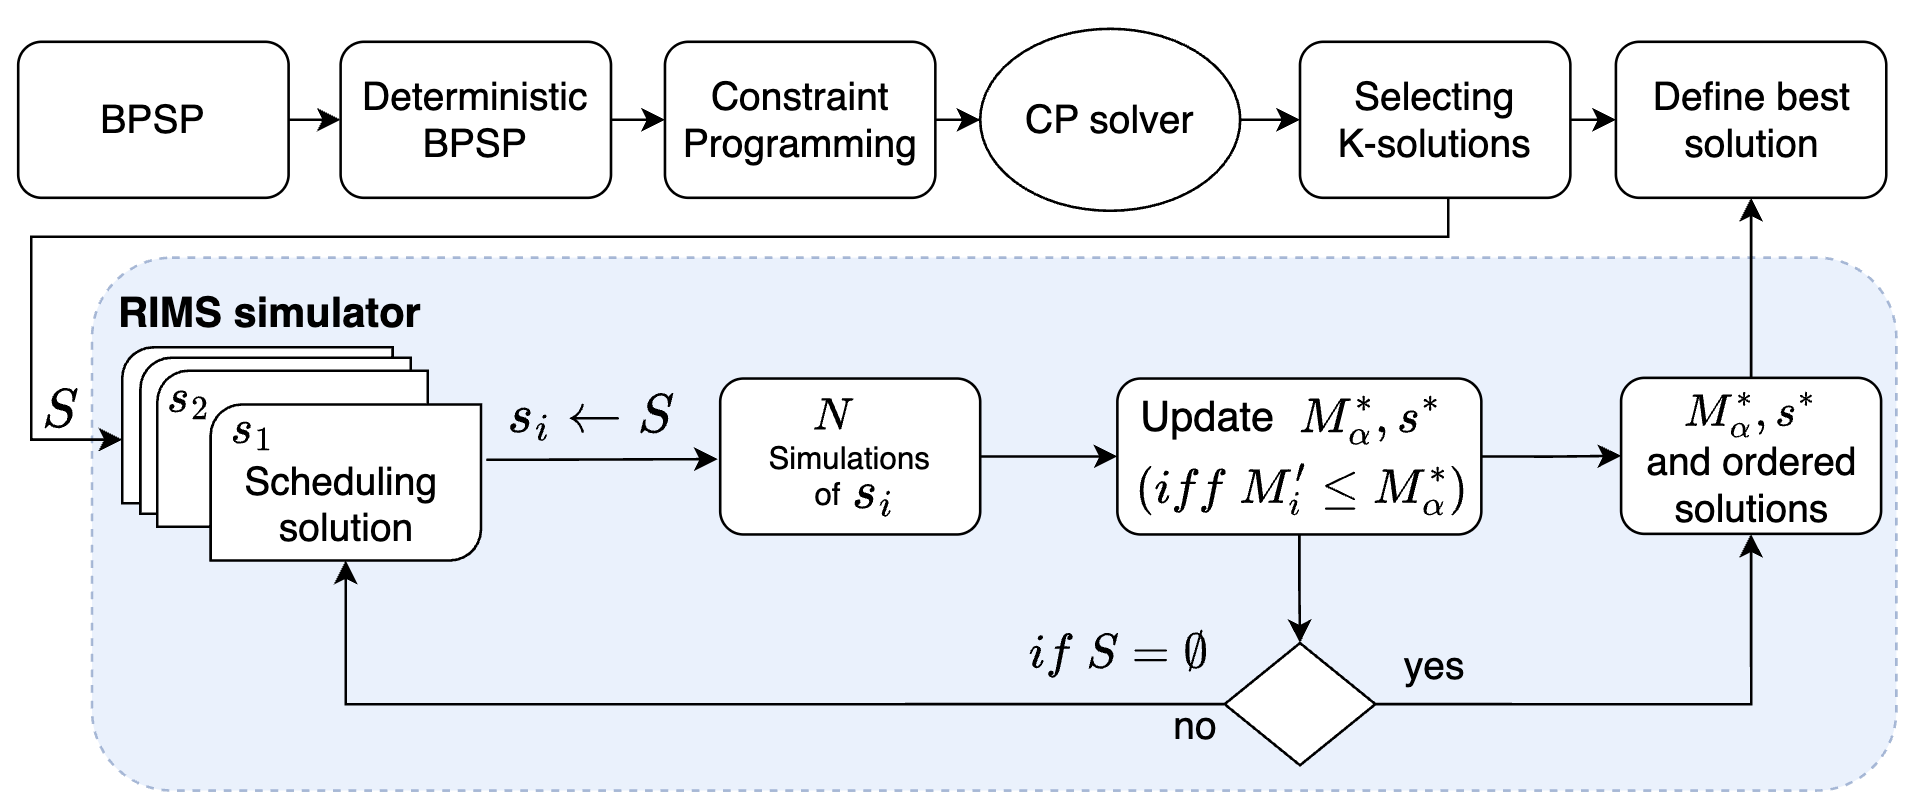
\includegraphics[width=\textwidth]{pipeline_rims3.png}
      \vspace{0.1cm}
      \scriptsize
      (Preview) We build an end-to-end pipeline.
  \end{columns}

  \vspace{0.15cm}
  \scriptsize
  \color{darkgray}
  Representative foundations: RCPSP / proactive scheduling (Beck \& Wilson), process mining (van der Aalst), scheduling textbooks (Pinedo).
\end{frame}

\begin{frame}{The gap we target (and the design principle)}
  \begin{columns}[T]
    \column{0.55\textwidth}
      \begin{block}{Gap}
        Business processes add two friction points that break ``standard'' scheduling:
        \begin{itemize}
          \item \btext{planned resource unavailability} (calendars)
          \item \btext{parameter extraction} from logs (durations, variability, resources)
        \end{itemize}
      \end{block}
      \begin{block}{Design principle}
        \btext{Optimize} deterministically (CP) \;+\; \btext{validate} under uncertainty (simulation).
      \end{block}

    \column{0.45\textwidth}
      \centering
      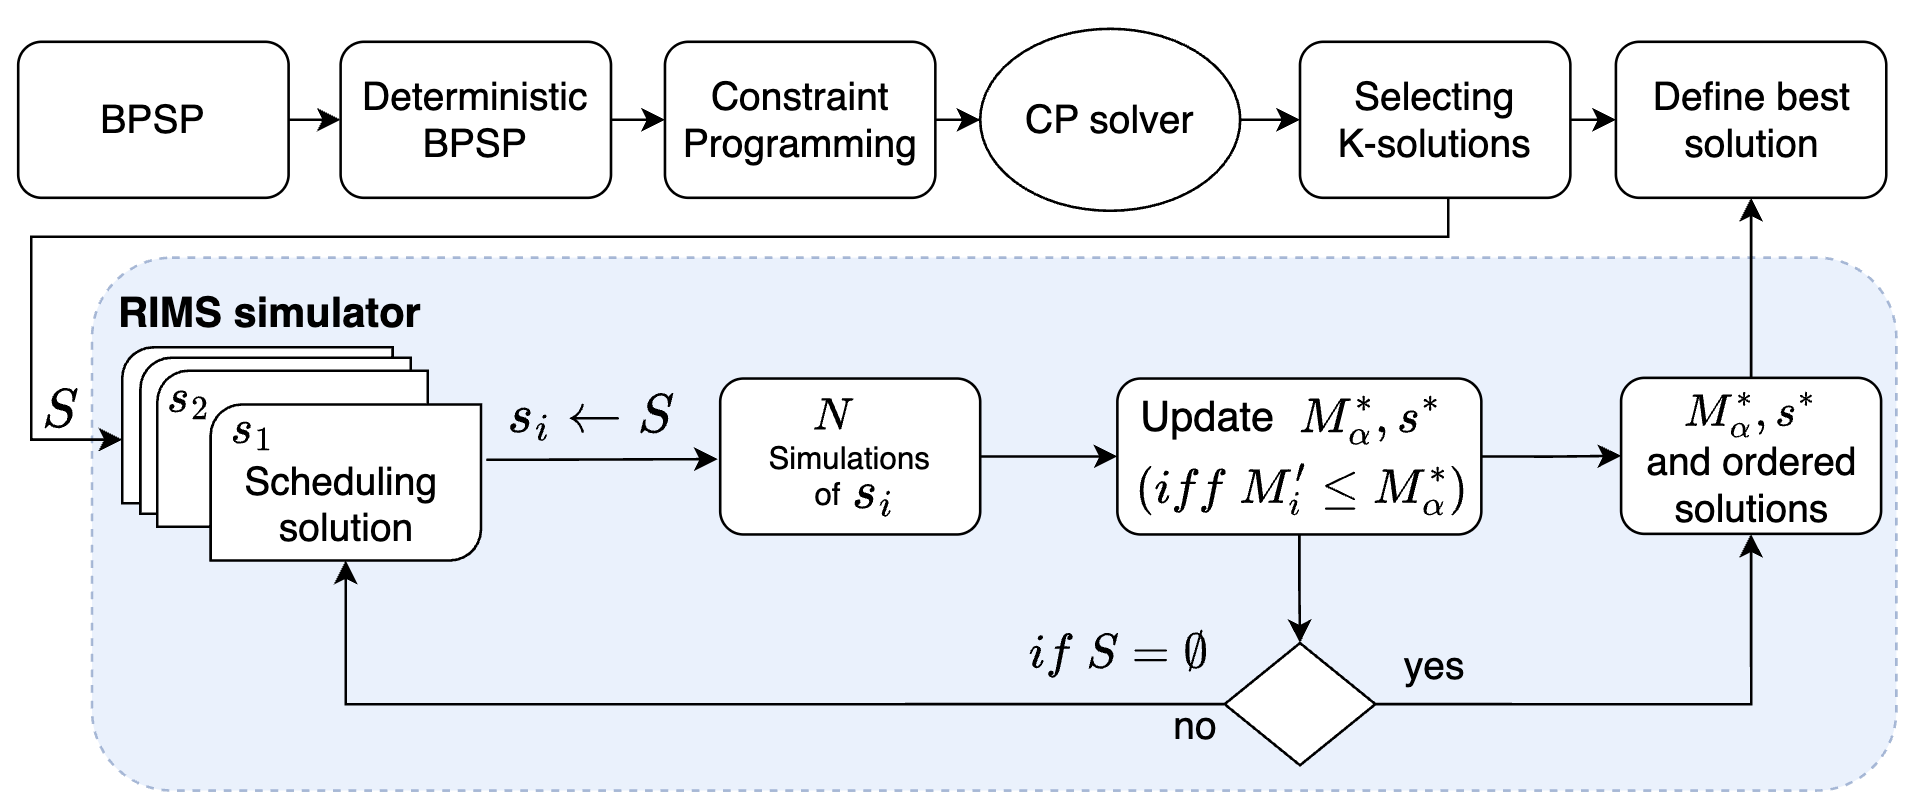
\includegraphics[width=\textwidth]{pipeline_rims3.png}
      \vspace{0.1cm}
      \scriptsize
      End-to-end pipeline (paper figure).
  \end{columns}
\end{frame}

\begin{frame}{Stochastic to deterministic: ``mean + buffer''}
  \begin{columns}[T]
    \column{0.62\textwidth}
      Turn random durations into deterministic ones:
      \[
        d = \mu + q \cdot \sigma
      \]
      \begin{itemize}
        \item \(q\) controls robustness: higher \(q\) \(\Rightarrow\) more buffer.
        \item With a principled \(q\), deterministic makespan lower-bounds the probabilistic objective.
      \end{itemize}

      \vspace{0.2cm}
      \btext{Slide placeholder (optional)}:
      add a small visual of a distribution with shaded tail (generate in ChatGPT UI).

    \column{0.38\textwidth}
      \centering
      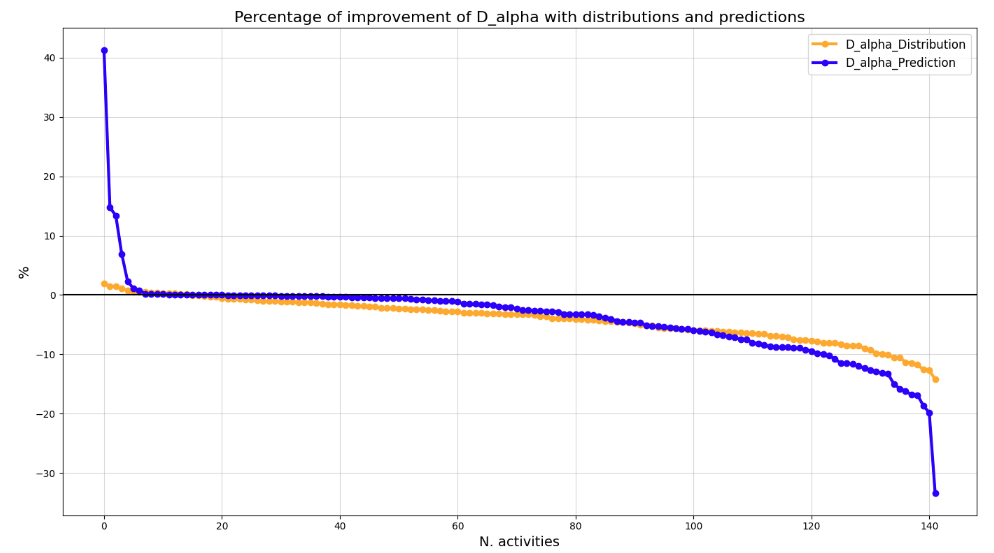
\includegraphics[width=\textwidth]{distribution_predictions.png}
      \scriptsize
      (Paper figure) durations as distributions rather than point estimates.
  \end{columns}
\end{frame}

\begin{frame}{Calendars matter: planned unavailability as constraints}
  \begin{columns}[T]
    \column{0.58\textwidth}
      In CP, resources are not continuously available.
      \begin{itemize}
        \item ``Unavailable'' periods block execution.
        \item Schedule must respect both \btext{capacity} and \btext{calendar} feasibility.
        \item Practical viewpoint: treat vacations as fixed ``dummy intervals'' that must not overlap.
      \end{itemize}

      \vspace{0.2cm}
      \btext{Recommendation}: include a simple calendar strip (work hours) for one resource.

    \column{0.42\textwidth}
      \centering
      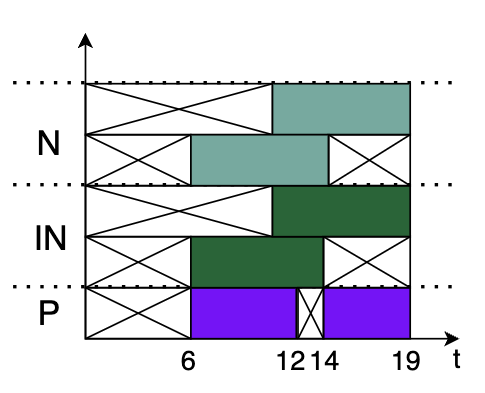
\includegraphics[width=\textwidth]{calendars.png}
      \scriptsize
      Example resource calendars (paper figure).
  \end{columns}
\end{frame}

\begin{frame}{Why CP + top-$K$ + Monte Carlo?}
  \begin{itemize}
    \item CP is strong at generating high-quality deterministic schedules quickly.
    \item But the probabilistic objective is only observable through simulation.
    \item So: solve deterministic, keep \btext{top-$K$} candidates, then select by Monte Carlo.
  \end{itemize}

  \vspace{0.3cm}
  \begin{block}{Takeaway}
    Use optimization to \btext{search}, simulation to \btext{judge} robustness.
  \end{block}
\end{frame}

\begin{frame}{Empirical note: choosing \(q\) (two options)}
  \begin{columns}[T]
    \column{0.52\textwidth}
      Two ways to set \(q\):
      \begin{itemize}
        \item \btext{Theoretical} \(q_U\): lower-bound guarantee.
        \item \btext{Data-driven} \(q_C\): estimate critical path via simulation; often tighter.
      \end{itemize}
      \vspace{0.2cm}
      In practice: \(q_C\) improves correlation, speeds up candidate selection.

    \column{0.48\textwidth}
      \centering
      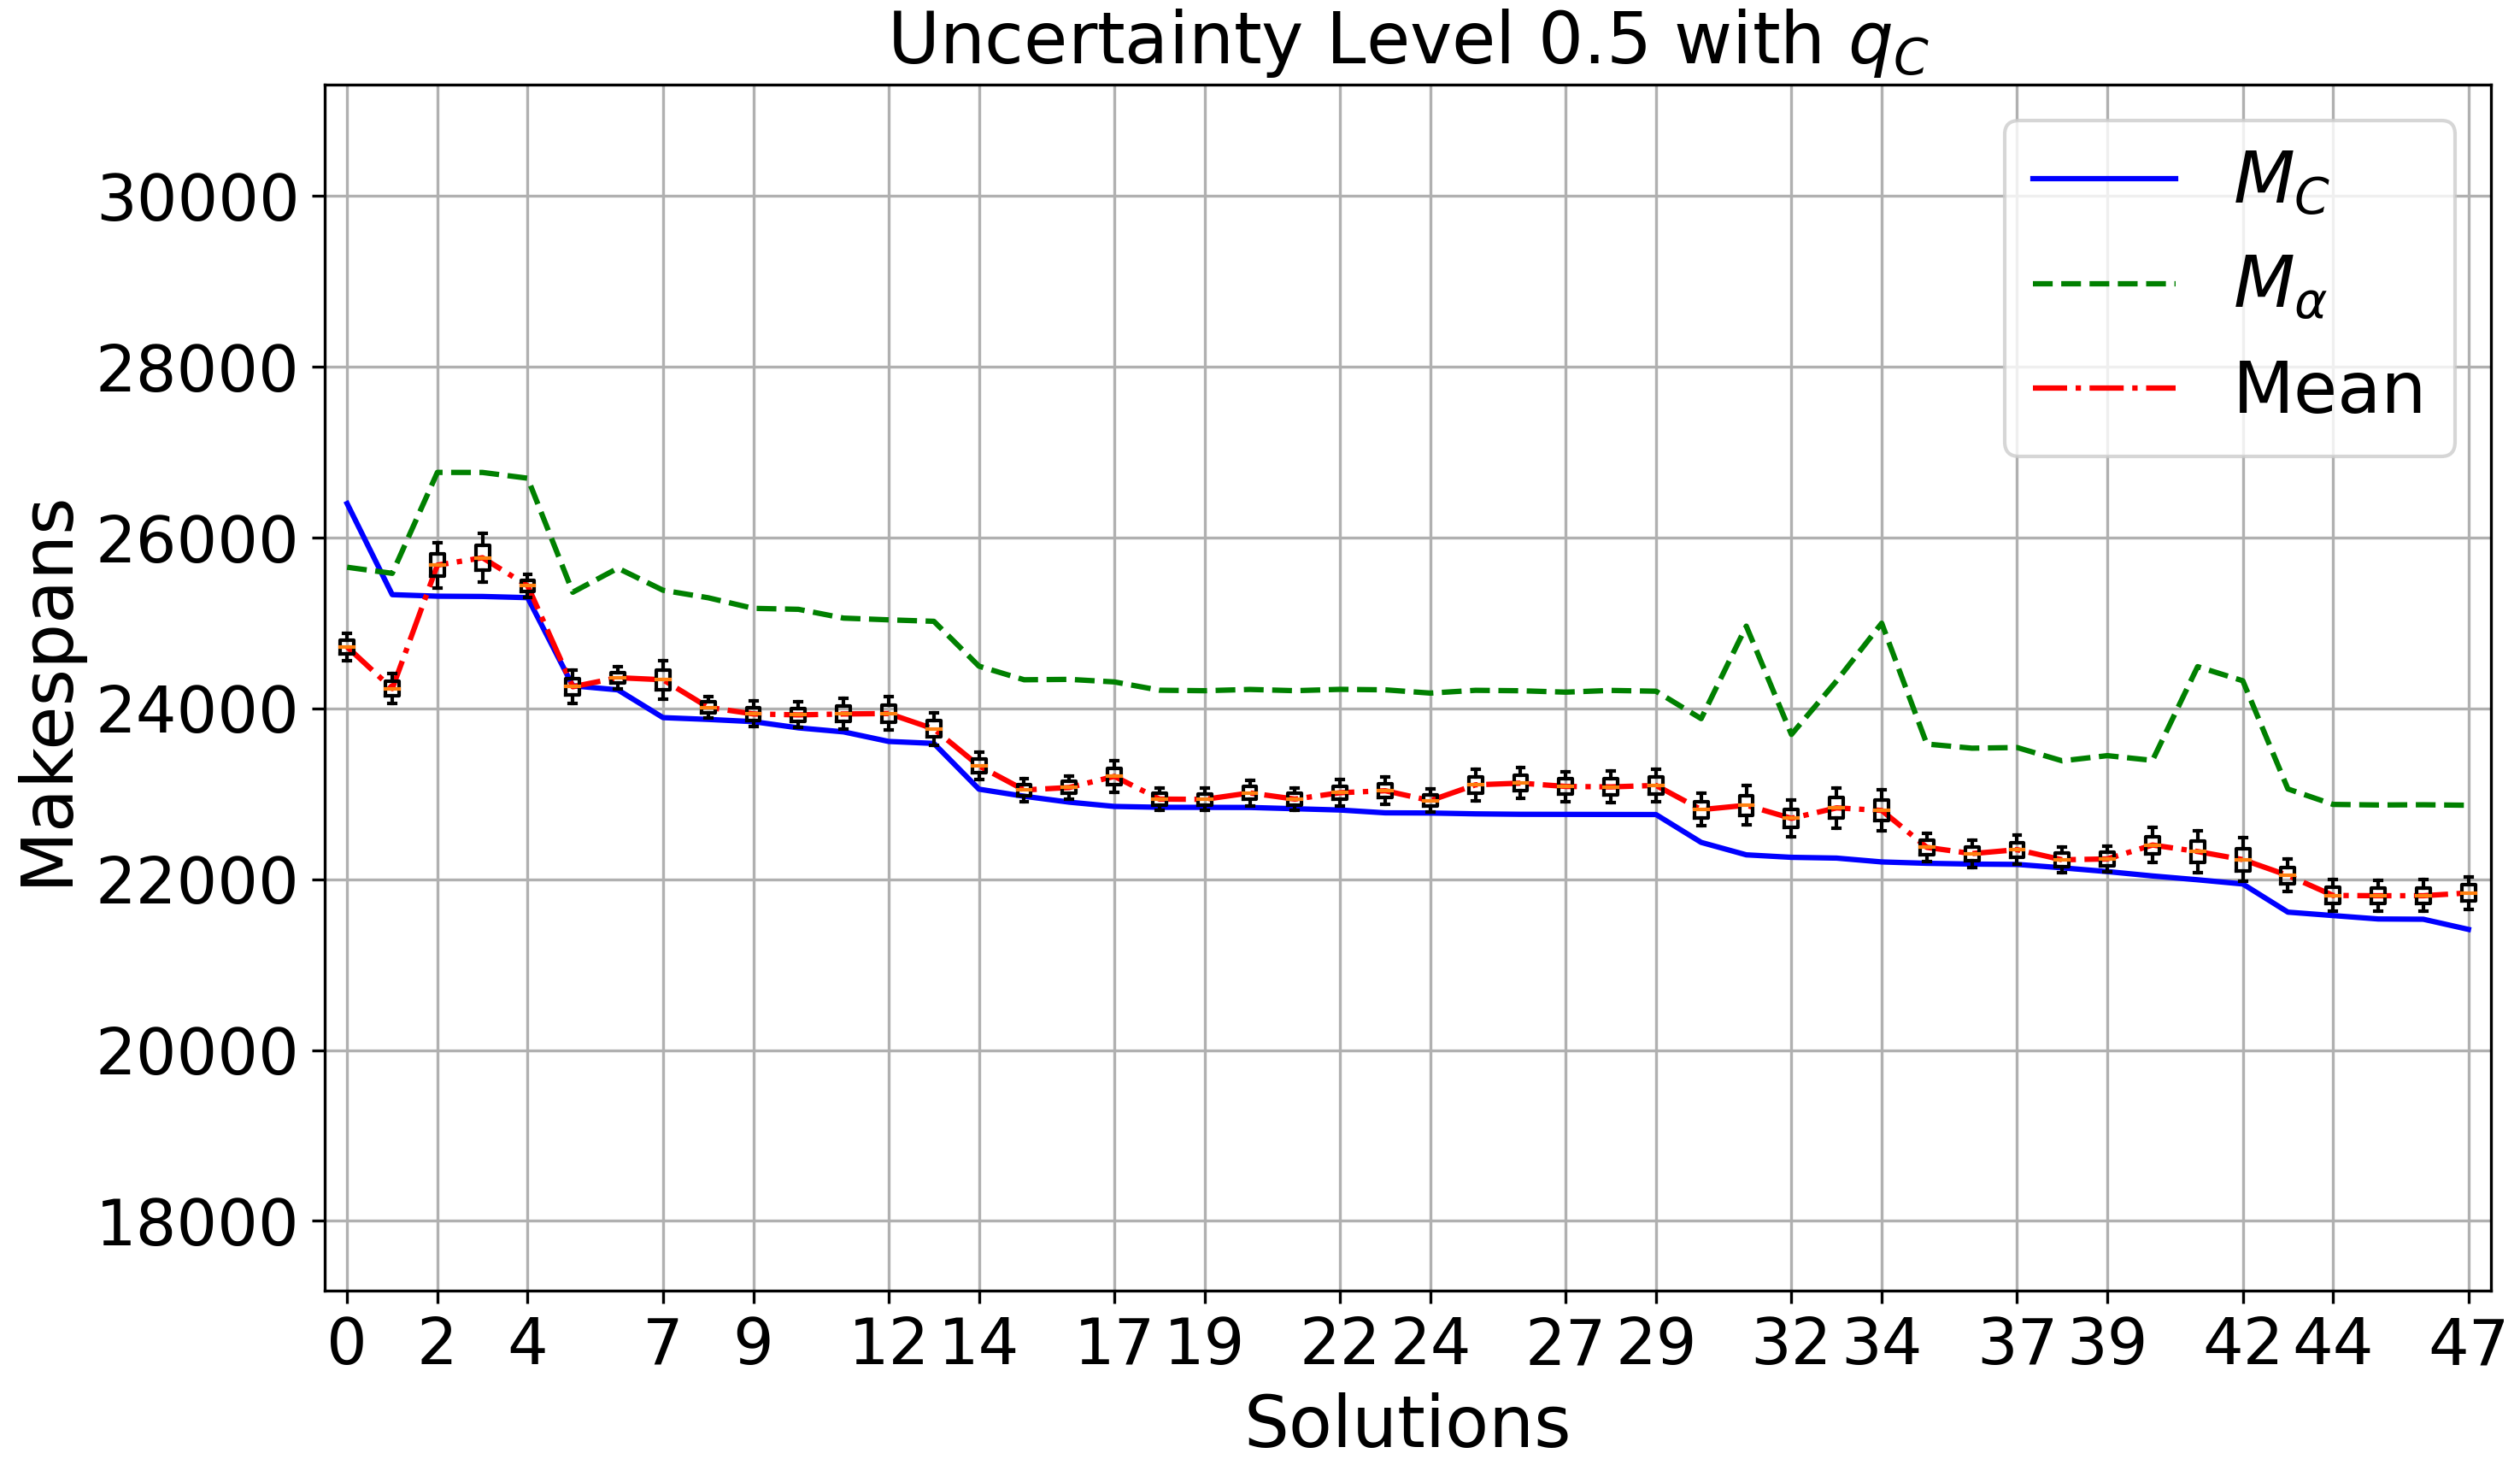
\includegraphics[width=\textwidth]{uncertainty_caledars_2.png}
      \scriptsize
      (Paper figure) deterministic vs probabilistic makespans across solutions.
  \end{columns}
\end{frame}

\begin{frame}{Real-world case: DayHospital (healthcare)}
  \begin{columns}[T]
    \column{0.62\textwidth}
      \btext{Setting}:
      \begin{itemize}
        \item High-volume day hospital operations
        \item Many patients (cases), many activities, many resources with calendars
        \item Fit parameters from 2021 logs; optimize schedules for held-out months
      \end{itemize}

      \vspace{0.2cm}
      \btext{Outcome}:
      \begin{itemize}
        \item average makespan improvement: \btext{5\%--14\%}
        \item up to \(\approx\) \btext{4 hours} reduction on busy days (reported)
      \end{itemize}

    \column{0.38\textwidth}
      \centering
      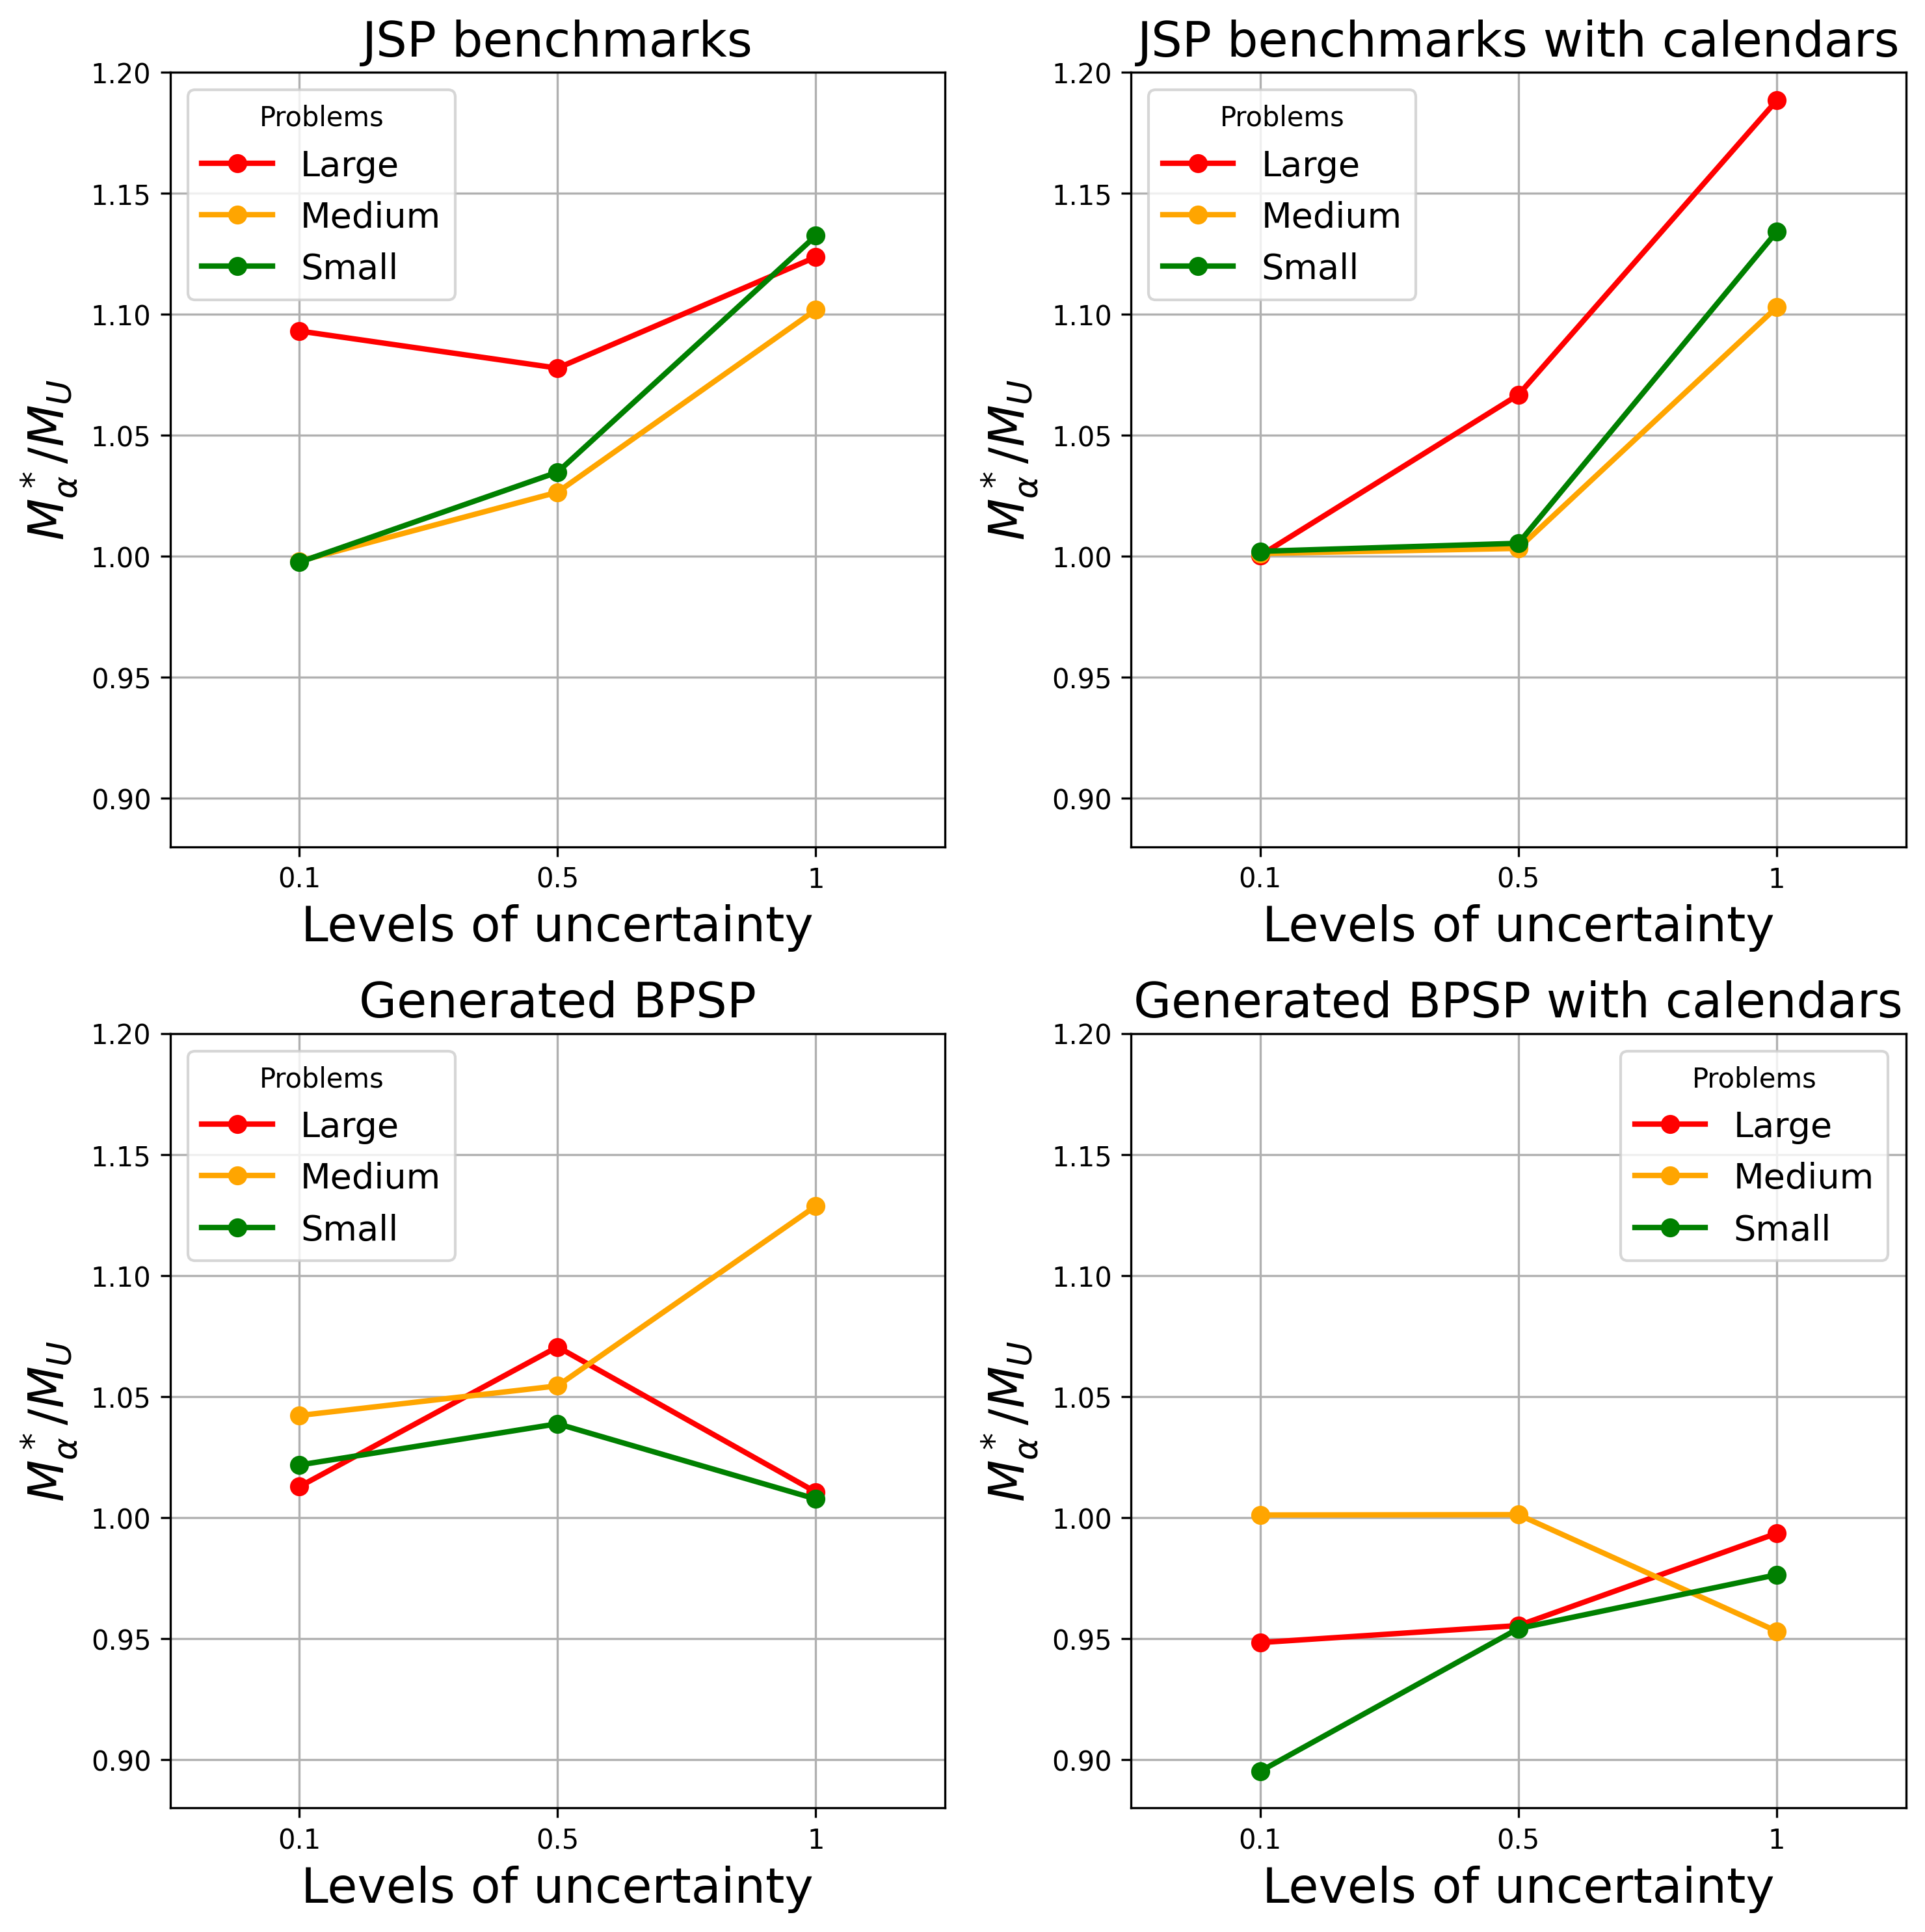
\includegraphics[width=\textwidth]{synthetic_exp.png}
      \scriptsize
      Placeholder: use this space for a clean ``before vs after'' Gantt snapshot later.
  \end{columns}
\end{frame}

\begin{frame}{What this gives BPO practitioners}
  \begin{columns}[T]
    \column{0.62\textwidth}
      \begin{block}{Operational value}
        \begin{itemize}
          \item robust appointment / release plans under uncertainty
          \item explicit use of resource calendars (a real pain point)
          \item data-driven: parameters extracted from logs, not ``assumed''
        \end{itemize}
      \end{block}

      \begin{block}{Scientific message}
        \btext{Scheduling is not just OR}---it is \btext{BPM-aware} and \btext{data-aware}.
      \end{block}

    \column{0.38\textwidth}
      \centering
      % Placeholder for a "deployment diagram" later:
      \fbox{\parbox{0.95\textwidth}{
        \vspace{0.15cm}
        \centering
        \textbf{Placeholder figure}\\
        Process mining $\rightarrow$ digital twin $\rightarrow$ scheduler\\
        \vspace{0.15cm}
      }}
      \vspace{0.1cm}
      \scriptsize
      Suggestion: generate a simple pipeline iconography in ChatGPT UI.
  \end{columns}
\end{frame}

% ---- Marker: TU/e cut line ----
% ==========================================================
% If you want the TU/e talk to be a strict prefix, stop after this section.
% Suggested TU/e stopping point: after "Predict-and-Schedule (real case)" slide below.
% ==========================================================

% ==========================================================
% 3) IJCAI'26 Predict-and-Schedule (white-box surrogate)
% ==========================================================
\section{Lens 2: Learning to Schedule with SASS (Structure-Aware Surrogates)}

\begin{frame}{Learning to schedule: research landscape}
  \begin{columns}[T]
    \column{0.62\textwidth}
      \begin{block}{Common paradigms}
        \begin{itemize}
          \item \btext{Predict-then-optimize}: learn durations (MSE), then apply a rule (SPT/EDD/FIFO)
          \item \btext{Learn-to-rank (LTR)}: learn an ordering surrogate, not the scheduling objective
          \item \btext{SPO / decision-focused learning}: train predictors to reduce downstream regret
        \end{itemize}
      \end{block}

      \begin{block}{The pain point in scheduling}
        The mapping from predictions to the schedule is \btext{discrete and brittle}:
        tiny prediction changes can flip critical decisions and cause large objective jumps.
      \end{block}

    \column{0.38\textwidth}
      \centering
      \fbox{\parbox{0.95\textwidth}{
        \vspace{0.2cm}
        \centering
        \textbf{Placeholder mini-visual}\\
        ``two jobs swap $\Rightarrow$ big SCT jump''\\
        \vspace{0.2cm}
      }}
      \vspace{0.1cm}
      \scriptsize
      Suggestion: generate a 2-job swap cartoon in ChatGPT UI.
  \end{columns}

  \vspace{0.1cm}
  \scriptsize
  \color{darkgray}
  Representative: SPO (Elmachtoub \& Grigas), learning-to-rank, classic scheduling (Pinedo).
\end{frame}

\begin{frame}{The Predict-then-Optimize disconnect}
  \begin{columns}[T]
    \column{0.5\textwidth}
      \begin{block}{Prediction (ML)}
        Learn durations \(\hat{y}\) by minimizing MSE:
        \[
          \min \sum (\hat{y}-y)^2
        \]
        \vspace{-0.2cm}
        \begin{itemize}
          \item good numeric accuracy
          \item \btext{blind to how predictions are used}
        \end{itemize}
      \end{block}

    \column{0.5\textwidth}
      \begin{block}{Scheduling (OR/AI)}
        Objective depends on \btext{order}, not values:
        \begin{itemize}
          \item SPT sorts by \(\hat{y}\)
          \item small errors can flip pairs
          \item flips can have \btext{large downstream cost}
        \end{itemize}
      \end{block}
  \end{columns}

  \vspace{0.25cm}
  \btext{Goal:} learn predictors that minimize \emph{decision regret} (schedule quality), not just MSE.
\end{frame}

\begin{frame}{SASS: structure-aware surrogates from critical decisions}
  \begin{itemize}
    \item Many deterministic optima are \btext{polynomial-time rules} that are \btext{discrete} but \btext{structured}:
    \begin{itemize}
      \item SPT: pairwise comparisons \(i \prec j\)
      \item Johnson: group assignment + within-group ordering
      \item EDD/FIFO: thresholding / sorting
    \end{itemize}
    \item \btext{SASS idea}: replace each critical decision by a smooth sigmoid penalty,
    and \btext{weight} it by its local impact on the objective.
    \[
      L_{\mathrm{surr}} = \sum_{d \in \mathcal{K}} \phi_d(\theta^\star)\,
      \sigma\!\left(\frac{-m_d}{\lambda}\right)
    \]
    where \(\phi_d\) is the \btext{cost of getting decision \(d\) wrong}.
  \end{itemize}

  \vspace{0.2cm}
  \btext{Recommendation}: add one animated example of a swapped pair (generate in UI).
\end{frame}

\begin{frame}{Instantiation: Single-machine SCT via SPT (one slide, high signal)}
  \btext{Objective:} minimize sum of completion times (SCT).

  \vspace{0.2cm}
  \btext{Deterministic optimum:} SPT (sort by true durations).

  \vspace{0.2cm}
  \btext{Critical decisions:} for each pair \((i,j)\), did we order them correctly?

  \vspace{0.2cm}
  \btext{Weight = cost of misordering:}
  \[
    R_{i,j} = (j-i)\,(y_j - y_i)
  \]

  \vspace{0.2cm}
  \btext{Loss:} penalize misordered pairs smoothly, proportional to \(R_{i,j}\).
\end{frame}

\begin{frame}{Results: synthetic evaluation (stability + scalability)}
  \begin{center}
    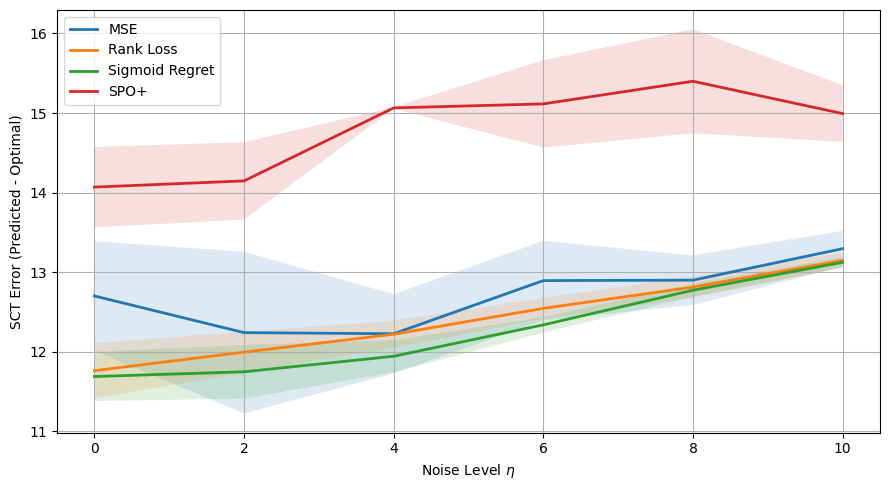
\includegraphics[width=0.48\textwidth]{new_plot/linearDataset_problem1.png}\hfill
    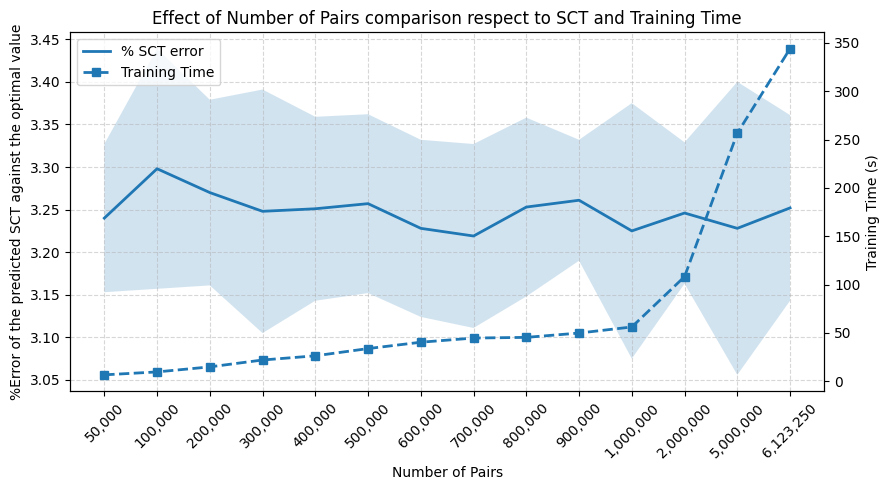
\includegraphics[width=0.48\textwidth]{new_plot/analysis_number_of_pairs.png}
  \end{center}
  \vspace{-0.1cm}
  \begin{itemize}
    \item \btext{Stability}: SASS is more stable than SPO+ under increasing noise.
    \item \btext{Scalability}: pairwise sampling is sufficient (e.g., \(\sim10{,}000\) pairs can already reach low SCT error).
  \end{itemize}
\end{frame}

\begin{frame}{Real-world: DayHospital outpatient scheduling (sequencing exams)}
  \begin{columns}[T]
    \column{0.58\textwidth}
      \btext{Setting}:
      \begin{itemize}
        \item outpatient exams (single-resource sequencing per day)
        \item durations uncertain; features from logs
        \item objective: reduce congestion (SCT)
        \item evaluation over \btext{Jan--Dec 2021} (one full year)
      \end{itemize}
      \vspace{0.2cm}
      \btext{Why it matters to BPM}:
      \begin{itemize}
        \item predictions are not the end goal
        \item the goal is \btext{better schedules} (patient experience + throughput)
      \end{itemize}

    \column{0.42\textwidth}
      \centering
      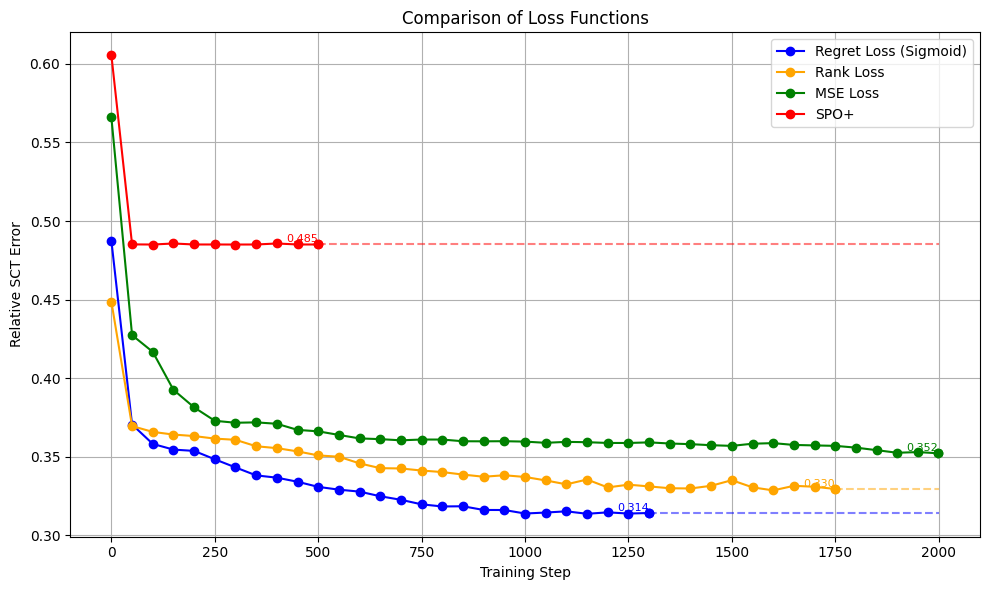
\includegraphics[width=\textwidth]{LossComparison_Jan.png}
      \scriptsize
      Example training dynamics on one month (paper figure).
  \end{columns}
\end{frame}

\begin{frame}{DayHospital results (headline slide)}
  \begin{columns}[T]
    \column{0.62\textwidth}
      \begin{block}{Key findings}
        \begin{itemize}
          \item \btext{Best in 11/12 months} (lowest relative SCT error)
          \item \btext{Average relative SCT error}: \btext{0.316} (SASS)
          \item Baselines (avg): 0.353 (MSE), 0.338 (LTR), 0.476 (SPO+)
          \item Improvement: \(\sim\)10\% vs MSE, \(\sim\)34\% vs SPO+
        \end{itemize}
      \end{block}
      \vspace{0.1cm}
      \btext{Interpretation:} learning is guided by the scheduling rule’s structure and the real cost of mistakes.

      \ifshort
        \vspace{0.15cm}
        \btext{(TU/e stop here)}: wrap up + Q/A.
      \fi

    \column{0.38\textwidth}
      \centering
      % Placeholder for a clean summary graphic later (bar chart or table screenshot).
      \fbox{\parbox{0.95\textwidth}{
        \vspace{0.15cm}
        \centering
        \textbf{Placeholder}\\
        12-month plot (Jan--Dec 2021)\\
        Relative SCT error by method\\
        \vspace{0.15cm}
      }}
      \vspace{0.1cm}
      \scriptsize
      Suggestion: generate a clean 12-month bar chart (or heatmap table) in ChatGPT UI.
  \end{columns}
\end{frame}

\ifshort
  % Short talk ends here (TU/e).
  \begin{frame}{Takeaways \& discussion}
    \begin{itemize}
      \item \btext{BPSP}: robust proactive schedules from logs + calendars improve real operations.
      \item \btext{Predict-and-schedule}: learn predictions that directly minimize scheduling regret.
      \item \btext{Open question}: how to generalize these ideas to richer BPM control-flow.
    \end{itemize}
    \vspace{0.35cm}
    \btext{Thank you.} \quad \small Questions / collaborations welcome.
  \end{frame}
  \end{document}
\fi

\begin{frame}{One more problem: Johnson’s rule (why it generalizes)}
  \begin{itemize}
    \item Two-machine flow shop \(F2\|C_{\max}\): Johnson’s rule is optimal when times are known.
    \item Rule decomposes into:
      \begin{itemize}
        \item \btext{grouping} decision (\(p_{1} < p_{2}\) vs \(p_{1} \ge p_{2}\))
        \item \btext{within-group ordering}
      \end{itemize}
    \item Same recipe: build smooth losses for each critical decision, weighted by swap costs.
  \end{itemize}
  \vspace{0.2cm}
  \btext{Message:} we can derive \emph{interpretable, stable} decision-focused learning objectives from classical algorithms.
\end{frame}

% ==========================================================
% 4) Teaser: OR gateways / externalities (one slide)
% ==========================================================
\section{Teaser: why OR gateways break local dispatching}

\begin{frame}{Teaser: OR gateways create synchronization externalities (why FIFO can fail)}
  \begin{columns}[T]
    \column{0.5\textwidth}
      \centering
      \scriptsize \textbf{FIFO at each queue (locally ``fair'')}
      \vspace{0.1cm}
      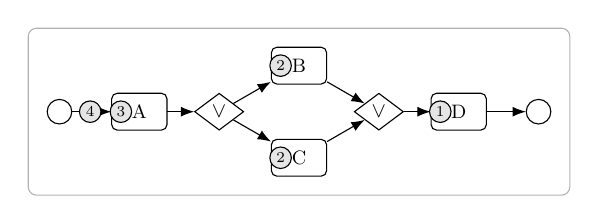
\begin{tikzpicture}[
        scale=0.78, every node/.style={transform shape},
        >=Latex,
        event/.style={circle,draw,minimum size=4mm},
        gateway/.style={diamond,draw,aspect=2.4,minimum width=8mm,minimum height=6mm,inner sep=0pt,line width=0.4pt},
        activity/.style={rectangle,draw,rounded corners=2pt,minimum width=9mm,minimum height=6mm,font=\small},
        case/.style={circle,draw,fill=black!10,inner sep=0.5pt,minimum size=3.5mm,font=\scriptsize}
      ]
        \node[event]    (start) at (0,0) {};
        \node[activity] (A)     at (1.3,0) {A};
        \node[gateway]  (split) at (2.6,0) {};
        \node[activity] (B)     at (3.9,0.75) {B};
        \node[activity] (C)     at (3.9,-0.75) {C};
        \node[gateway]  (join)  at (5.2,0) {};
        \node[activity] (D)     at (6.5,0) {D};
        \node[event]    (end)   at (7.8,0) {};
        \node at (split.center) {$\vee$};
        \node at (join.center)  {$\vee$};
        \draw[->] (start) -- (A);
        \draw[->] (A) -- (split);
        \draw[->] (split) -- (B);
        \draw[->] (split) -- (C);
        \draw[->] (B) -- (join);
        \draw[->] (C) -- (join);
        \draw[->] (join) -- (D);
        \draw[->] (D) -- (end);
        % cases (visual cue only)
        \node[case] at (6.2, 0.00) {1};
        \node[case] at (3.6, 0.75) {2};
        \node[case] at (3.6,-0.75) {2};
        \node[case] at (1.0, 0.00) {3};
        \node[case] at (0.5, 0.00) {4};
        \draw[gray!60, rounded corners=3pt]
          ($(current bounding box.south west)+(-0.3,-0.3)$)
          rectangle
          ($(current bounding box.north east)+(0.3,0.3)$);
      \end{tikzpicture}

    \column{0.5\textwidth}
      \begin{block}{What breaks?}
        In OR/AND gateways, completion requires \btext{synchronization}.\\
        Local choices at \(B\) and \(C\) can delay others at the join:
        \begin{itemize}
          \item \btext{delay externalities} across branches
          \item FIFO can be locally fair but globally inefficient
        \end{itemize}
      \end{block}
      \begin{block}{Pointer}
        Our IJCAI'26 work: \btext{value-of-time} reporting + VCG-style pricing
        to reconcile \btext{efficiency} and \btext{neutrality}.
      \end{block}
  \end{columns}
\end{frame}

% ==========================================================
% Closing
% ==========================================================
\section{Wrap-up}

\begin{frame}{Three takeaways}
  \begin{enumerate}
    \item \btext{BPO scheduling is real:} calendars + uncertainty + routing are first-class.
    \item \btext{Robust proactive scheduling works:} CP + simulation + logs improve makespan in practice.
    \item \btext{Learning must be decision-aware:} train for schedule quality, using algorithm structure.
  \end{enumerate}

  \vspace{0.35cm}
  \begin{block}{Discussion / collaboration}
    Looking for: partner processes, event logs, and joint deployments of scheduling + learning in BPM systems.
  \end{block}

  \vspace{0.1cm}
  \small \color{darkgray}
  (Figures sourced from your chapter and IJCAI'25 / IJCAI'26 draft materials in this repository.)
\end{frame}

\end{document}

